\documentclass[10pt]{article}

\usepackage[version=3]{mhchem} % Package for chemical equation typesetting
\usepackage{siunitx} % Provides the \SI{}{} and \si{} command for typesetting SI units
\usepackage{graphicx} % Required for the inclusion of images
\usepackage{natbib} % Required to change bibliography style to APA
\usepackage{nth}
\usepackage{amsmath} % Required for some math elements
\usepackage{tabulary}
\usepackage{graphicx}
\usepackage{float}
\usepackage[font={small}]{caption}
\usepackage[margin=1in]{geometry}
\setlength\parindent{0pt} % Removes all indentation from paragraphs

\renewcommand{\labelenumi}{\alph{enumi}.} % Make numbering in the enumerate environment by letter rather than number (e.g. section 6)

%\usepackage{times} % Uncomment to use the Times New Roman font


\title{Glassware, \\ Precision \& Accuracy \\ CHEM 1211L} % Title

\author{Chris \textsc{West}} % Author name

\date{\today} % Date for the report

\begin{document}

\maketitle % Insert the title, author and date

\begin{center}
\begin{tabular}{l r}
Date Performed: & June 7, 2017 \\% Date the experiment was performed
Partner: & Chris Tillis \\ % Partner names
Instructor: & Dr. MacGowan % Instructor/supervisor
\end{tabular}
\end{center}


%----------------------------------------------------------------------------------------
%	SECTION 1
%----------------------------------------------------------------------------------------

\section{Experimental procedure}

\hspace{5ex}In, our experiment to determine the volume of an unmarked container. We were given a small glass ``Round Bottom Flask"(Figure 1) with a white cloud color around its neck that contained the words 25 ml marked in small bold white letters on its body. The other kinds of equipment that we used to carry out this experiment was a wash bottle (contained the water), electronic balance, clamp and stand, Graduated Cylinder, and Buret. \\

\begin{figure}[H]
\hfill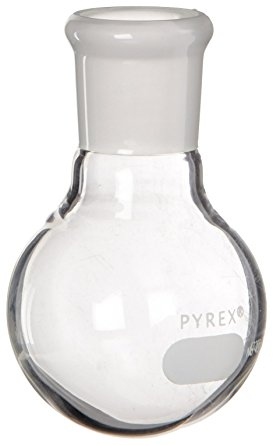
\includegraphics[width=1in]{figure1}\hspace*{\fill}
\caption[Round Bottom Flask]{Round Bottom Flask}
\end{figure}

\hspace{5ex}First, we weighed the empty Graduated Cylinder in grams. Then added water using the wash bottle to the Graduated Cylinder up to 34 ml. Then we take the round bottom flask and clamp it to the stand. We then took the water that was now in the Graduated Cylinder and added it to the round bottom flask. The water should then stop just right at where the white cloud around it's neck begins. If it doesn't, we dump the water out and start over from the beginning and change the measurement. If it does, then we dump the water back into the Graduated Cylinder and get the new weight. Subtract the new weight of the Graduated Cylinder from the old weight of the Graduated Cylinder and get the weight of the water. Then repeat this trial for a second time. \\

\hspace{5ex}After you have completed the steps above then we do another procedure. First, we weighed the empty Graduated Cylinder in grams. Then take a Buret and clamp it to the stand. Now we fill the Buret to the marking 1 ml. Place the empty Round Bottom Flask underneath the Buret. Then open the bottom of the Buret using the lever. Allow, water to drip into the Round Bottom Flask all the way to where the white cloud around it's neck begins. Pour the water from the Round Bottom Flask into the Graduated Cylinder and get the new weight. Subtract the new weight from the old weight and get the weight of the water in grams.\\
%----------------------------------------------------------------------------------------
%	SECTION 2
%----------------------------------------------------------------------------------------

\section{Collected Experimental Data}
\begin{table}[H]
\resizebox{20em}{!}{
\begin{tabular}{|l|l|l|}
\hline
\multicolumn{1}{|c|}{{\ul{\textbf{Trial run \#}}}} & \multicolumn{1}{c|}{{\ul{\textbf{ml of water measured}}}} \\ \hline
	1 & 34.0 \\ \hline
	2 & 34.0 \\ \hline
	\end{tabular}
	}
	\centering
\caption{Data Collected to Determine the Volume of Unknown Container Using our Procedure (Using Graduated Cylinder)}
\label{Table 1}
\end{table}

\begin{table}[H]
\resizebox{20em}{!}{
\begin{tabular}{|l|l|l|}
\hline
\multicolumn{1}{|c|}{{\ul{\textbf{Trial run \#}}}} & \multicolumn{1}{c|}{{\ul{\textbf{ml of water measured}}}} \\ \hline
	1 & 31.55 \\ \hline
	\end{tabular}
	}
	\centering
\caption{Data Collected to Determine the Volume of Unknown Container Using Instructor's Procedure (Using Buret)}
\label{Table 2}
\end{table}

\begin{table}[H]
\resizebox{20em}{!}{
\begin{tabular}{|l|l|l|}
\hline
\multicolumn{1}{|c|}{{\ul{\textbf{Trial run \#}}}} & \multicolumn{1}{c|}{{\ul{\textbf{ml of water measured}}}} \\ \hline
	1 & 31.28 (31.21 grams) \\ \hline
	\end{tabular}
	}
	\centering
\caption{Data Collected for Determining the Volume of Unknown Container - Gravimetrically}
\label{Table 2}
\end{table}
%----------------------------------------------------------------------------------------
%	SECTION 3
%----------------------------------------------------------------------------------------

\section{Calculations}
\hspace{5ex}Determining the average volume of unknown container:
\begin{center}
Avg. vol. = $\frac{(34.0 ml + 34.0 ml + 31.55 ml + 31.28 ml)}{4}$ = 32.7075 ml \\
Avg. vol. = 32.71 ml\\
\end{center}
\hspace{5ex}Determining volume by mass using density of water:
\begin{center}
D = $\frac{m}{v}$ \\
D = .9977 $\frac{g}{ml}$ \\
m = 31.21 g \\
v = ? \\

.9977 $\frac{g}{ml}$ = $\frac{31.21 g}{v}$ \\
v =  $\frac{\SI{31.21}{\gram}}{.9977 g}$ ml = 31.28 ml \\
\end{center}
\hspace{5ex}Determine the difference error between our groups determined volume and volume determined by the gravimetric method:
\begin{center}
Difference error \% = ((experimental value - accepted value)/accepted value)) x 100 \\
experimental value = 34.0 ml\\
accepted value = 31.28 ml\\
difference error = ? \\
Difference error \% = ((34.0 ml - 31.28 ml)/31.28 ml)) x 100 = 8.695 \\
Difference error = 8.70 \%
\end{center}
%----------------------------------------------------------------------------------------
%	SECTION 3
%----------------------------------------------------------------------------------------

\section{Questions}
\hspace{5ex}Our precision of recorded measurements were determined by the Graduated Cylinder measured to the ml and the Buret measured to the \nth{10} of ml.

\hspace{5ex}The kind of errors we got were from the electronic balance that we subtracted from are calculations. This would be consider systematic because it was a sudden onset. A random possible occurrence could be the filling of the Graduated Cylinder then submitting the water from the Graduated Cylinder to the Round Bottom Flask. We most likely were not always accurately at the line we mentally made as a stop pointing for filling the glass container. \\

\hspace{5ex}Our groups communication of understanding the assignment at hand needs some improvement. We wrote out the directions but viewed them two completely different ways. So, communication from the start and explaining what we see to each other is crucially important. Once we were on same page are teamwork was great. Our pace and communication to one another was excellent. \\

\hspace{5ex}In image ``A," (figure 2) we have a Buret measured at 3.15 ml by looking at where the line sort of dips like a smile. For image ``B," (figure 3) its a Graduated Cylinder which is measured at 35.0 ml where the water line ends.\\
\begin{figure}[H]
\hfill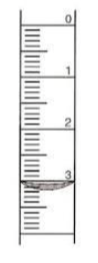
\includegraphics[width=.7in]{imageA}\hspace*{\fill}
\caption[Image A]{Image A}
\end{figure}
\begin{figure}[H]
\hfill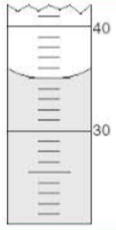
\includegraphics[width=.7in]{imageB}\hspace*{\fill}
\caption[Image B]{Image B}
\end{figure}
\end{document}
